\documentclass[lualatex,paper=a4paper,fontsize=10pt]{jlreq}

\usepackage[top=22mm,bottom=22mm,left=24mm,right=24mm]{geometry}

\usepackage{graphicx}
\usepackage{float}
\usepackage{amsmath}
\usepackage{listings}
\usepackage{booktabs}
\usepackage{array}
\usepackage{url}

\lstset{
  language=C,
  basicstyle=\ttfamily\footnotesize,
  numbers=left,
  numberstyle=\scriptsize,
  numbersep=8pt,
  frame=single,
  breaklines=true,
  columns=fullflexible,
  keepspaces=true,
  showstringspaces=false,
  tabsize=4,
  captionpos=b
}

\title{プログラミング レポート2}
\author{202512228 小松侑輝}
\date{2026年7月}

\begin{document}
\maketitle

\section{はじめに}
本レポートでは、標準入力から得た文字列を動的に確保したメモリへ保存するプログラムと、保存した文字列の一部を別の文字列へ置換するプログラムを作成した。実行時に必要な大きさのメモリを得るには \texttt{malloc} を用い、使用後には \texttt{free} で解放する必要がある。

課題の指示に従い、大域変数を使用しなかった。入力には \texttt{fgets} を用い、文字列の長さの取得には \texttt{strlen}、文字列のコピーには \texttt{strcpy}部分文字列の探索には \texttt{strstr} を用いた。動的メモリを確保する際には、文字列末尾のヌル文字の領域を含めるため、文字列長に 1 を加えた大きさを指定した。さらに、\texttt{malloc} の返り値が \texttt{NULL} でないことを必ず確認した。

\section{設問1}
\subsection{設問内容の理解と実装方針}
設問1では、動的に確保したメモリ上の文字列を最大100個保存し、入力終了後に3桁の行番号を付けて表示する。そこで、文字列そのものを固定長の二次元配列へ保存するのではなく、文字列の先頭アドレスを格納する \texttt{char*} 型の配列 \texttt{lines} を用意する。入力時には一時的な文字配列 \texttt{buf} に \texttt{fgets} で1行を読み込む。読み込んだ文字列の先頭3文字が \texttt{...} であれば保存せずに入力を終了する。

通常の文字列であれば、\texttt{strlen(buf)+1} バイトを \texttt{malloc} で確保し、\texttt{strcpy} で内容をコピーする。この方法では、各行について実際に必要な最小限のメモリだけを確保できる。入力終了後は、書式指定 \texttt{\%03d} を用いて行番号を常に3桁で表示し、最後に確保したすべての領域を \texttt{free} で解放する。

\subsection{作成したプログラムとポイント}
作成したプログラムをリスト\ref{lst:q1}に示す。

\lstinputlisting[caption={設問1のプログラム（s2512228-1.c）},label={lst:q1}]{s2512228-1.c}

リスト\ref{lst:q1}の9行目では、100個の文字列のアドレスを保存する配列を宣言している。16行目の繰り返し条件を \texttt{n < LINES} とすることで、配列の範囲外へ書き込まないようにした。21行目では短絡評価を利用し、先頭から3文字がすべてピリオドである場合に入力を終了している。

25行目では、読み込んだ文字列の長さにヌル文字の1バイトを加えた大きさを確保している。26--32行目では \texttt{malloc} の失敗を確認し、失敗した場合にはそれまでに確保した領域を解放してから異常終了する。34--36行目で文字列を確保領域へコピーし、その先頭アドレスを \texttt{lines} に保存する。39--45行目では行番号を3桁で表示する。通常は入力文字列に改行コードが含まれるが、バッファの上限まで入力された場合にも次の行と連結しないよう、末尾に改行がない場合は追加で改行を出力するようにした。47--49行目では、全行の表示後に確保領域を解放している。

\subsection{確認方法と結果}
コンパイルは次のコマンドで行った。

\begin{lstlisting}[numbers=none]
gcc -std=c89 -o s2512228-1.exe s2512228-1.c
\end{lstlisting}

作成したプログラムに対して、alpha、beta、gammaの3行を入力し、
その後に終了条件である「...」を入力した。
実行結果を図\ref{fig:result1}に示す。

\begin{figure}[H]
  \centering
  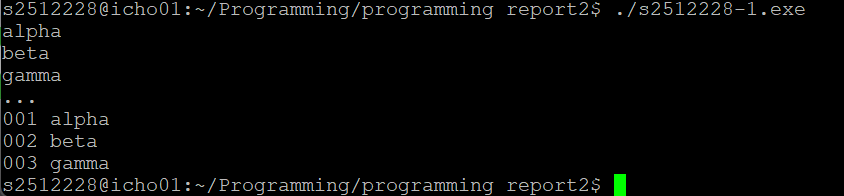
\includegraphics[width=0.9\linewidth]{result1.png}
  \caption{設問1の実行結果}
  \label{fig:result1}
\end{figure}

図\ref{fig:result1}より、入力した3行が001から始まる3桁の行番号付きで
正しく表示されることを確認した。

また、100行の文字列を入力し、最後まで正しく保存・表示できるかを確認した。
実行結果の末尾を図\ref{fig:result100}に示す。

\begin{figure}[H]
  \centering
  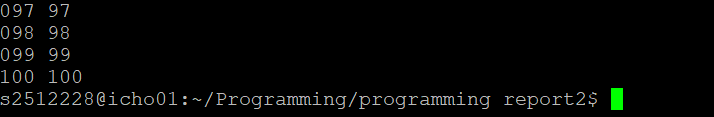
\includegraphics[width=0.7\linewidth]{result2.png}
  \caption{100行入力した場合の実行結果の末尾}
  \label{fig:result100}
\end{figure}

図\ref{fig:result100}より、行番号097から100までが正しく3桁で表示され、
100行目まで処理した後にプログラムが終了することを確認した。以上より、終了条件、最大個数、行番号の書式、動的メモリの確保と解放が設問の条件を満たしていると判断した。

\section{設問2}
\subsection{設問内容の理解と実装方針}
設問2では、設問1で保存した各行について、置換元の文字列 \texttt{s} が含まれていれば、その行で最初に現れる \texttt{s} だけを置換後の文字列 \texttt{t} に変更する。この操作を、\texttt{s} または \texttt{t} の先頭が \texttt{...} となるまで繰り返す。

\texttt{fgets} で \texttt{s} と \texttt{t} を読み込むと、通常は末尾に改行コードが含まれる。そのままでは入力行中の文字列と一致しにくいため、講義ノートの演習で扱われた方法に従い、末尾の改行コードを削除する関数 \texttt{chomp} を用意した。各行における最初の出現位置は \texttt{strstr} で求める。見つかった位置のポインタを関数 \texttt{substitution} に渡し、置換前部分、\texttt{t}、置換後部分の順に1文字ずつ新しい領域へコピーする。

新しい文字列に必要な大きさは、
\[
  \text{元の長さ}-\texttt{s}\text{の長さ}+\texttt{t}\text{の長さ}+1
\]
である。最後の1はヌル文字の領域である。新しい文字列の作成に成功したら、古い行の領域を \texttt{free} し、\texttt{lines[i]} を新しい文字列のアドレスへ入れ替える。結果を確認しやすくするため、各置換操作の後に全行を表示する。

\subsection{作成したプログラムとポイント}
作成したプログラムをリスト\ref{lst:q2}に示す。

\lstinputlisting[caption={設問2のプログラム（s2512228-2.c）},label={lst:q2}]{s2512228-2.c}

8--17行目の \texttt{chomp} は、文字列の末尾が改行コードである場合に限って、その位置をヌル文字へ置き換える。19--30行目の \texttt{print\_lines} と32--38行目の \texttt{free\_lines} は、表示処理と解放処理の重複を避けるための関数である。いずれの関数も配列と要素数を引数で受け取るため、大域変数は使用していない。

40--81行目が置換後の文字列を作る \texttt{substitution} である。この関数内で呼び出している関数は、文字列長を求める \texttt{strlen} と領域を確保する \texttt{malloc} だけである。54行目の \texttt{position-old} は、元の文字列の先頭から置換位置までの文字数を表す。56行目で必要量を正確に計算して確保し、62--65行目で置換位置より前、67--70行目で \texttt{t}、72--77行目で \texttt{s} より後の部分をコピーする。78行目でヌル文字を置くことで、新しい文字列を正しく終端している。

116--147行目が置換を繰り返す処理である。119行目と126行目で改行を削除した後、それぞれの先頭が \texttt{...} であるか確認する。132行目の \texttt{strstr} が返すのは最初に一致した位置であるため、同じ行に \texttt{s} が複数存在しても最初の1か所だけが置換される。134行目で新しい文字列を作り、140行目で古い領域を解放してから141行目でアドレスを入れ替える。この順序により、元の文字列を破壊せずに新しい文字列を作成でき、使用しなくなった領域も残らない。

\subsection{確認方法と結果}
設問1と同様に、次のコマンドでコンパイルした。

\begin{lstlisting}[numbers=none]
gcc -std=c89 -o s2512228-2.exe s2512228-2.c
\end{lstlisting}

確認では、3行を保存した後、\texttt{pars} を \texttt{lex} に置換した．続いて、存在しない \texttt{zzz} を \texttt{yyy} に置換しようとした後、\texttt{...} を入力して終了した。主要部分の実行結果を次に示す。

\begin{figure}[H]
  \centering
  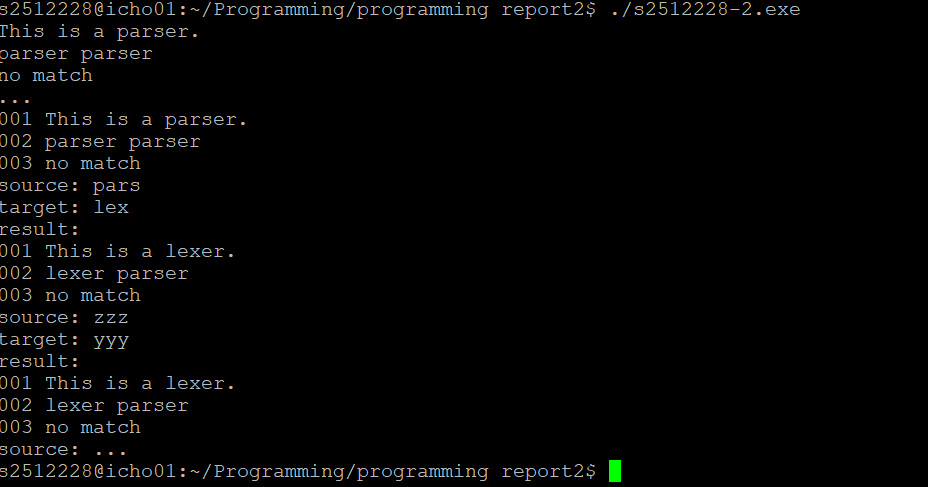
\includegraphics[width=0.85\linewidth]{result3.png}
  \caption{設問2における文字列置換の実行結果}
  \label{fig:result2}
\end{figure}

1行目では \texttt{parser} の \texttt{pars} が \texttt{lex} に置き換わり、\texttt{lexer} となった。2行目には \texttt{pars} が2回含まれているが、最初のものだけが置換されて \texttt{lexer parser} となった。また、\texttt{zzz} はどの行にも存在しないため、その後の一覧は変化しなかった。

さらに、置換文字列の長さに関する条件を表\ref{tab:q2test}のように確認した。

\begin{table}[htbp]
  \centering
  \caption{設問2の追加確認}
  \label{tab:q2test}
  \begin{tabular}{>{\raggedright\arraybackslash}p{35mm}p{45mm}p{65mm}}
    \toprule
    確認項目 & 入力例 & 確認結果 \\
    \midrule
    短い文字列への置換 & \texttt{abc} $\rightarrow$ \texttt{X} & \texttt{abc abc} は \texttt{X abc} となり，最初の1か所だけが置換された． \\
    長い文字列への置換 & \texttt{X} $\rightarrow$ \texttt{longertext} & 新しい長さに合わせて領域が確保され，文字列の欠落なく表示された． \\
    空文字列への置換 & \texttt{short} $\rightarrow$ 空文字列 & 該当部分が削除され，空の行として表示された． \\
    \bottomrule
  \end{tabular}
\end{table}

\begin{figure}[H]
  \centering
  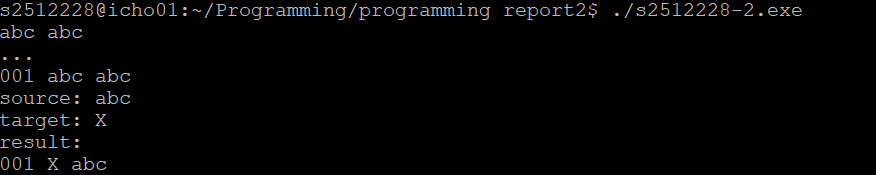
\includegraphics[width=0.85\linewidth]{result4.png}
  \caption{短い文字列へ置換した場合の実行結果}
  \label{fig:result4}
\end{figure}

\begin{figure}[H]
  \centering
  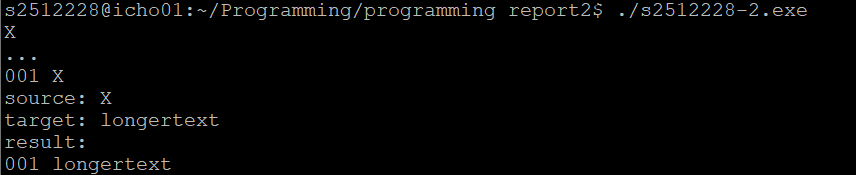
\includegraphics[width=0.85\linewidth]{result5.png}
  \caption{長い文字列へ置換した場合の実行結果}
  \label{fig:result5}
\end{figure}

\begin{figure}[H]
  \centering
  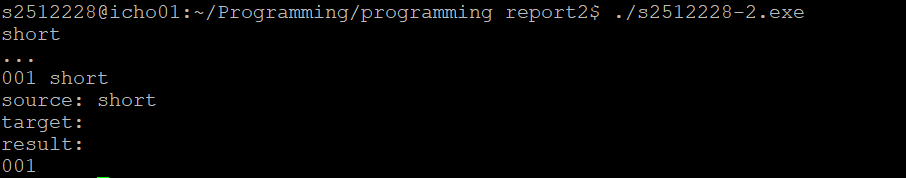
\includegraphics[width=0.85\linewidth]{result6.png}
  \caption{空文字列へ置換した場合の実行結果}
  \label{fig:result6}
\end{figure}

置換前後で文字列の長さが変わる場合にも、必要なメモリ量を式で計算しているため、固定長配列の大きさに依存せずに処理できた。また、置換が行われた行では古い領域を解放し、プログラム終了時には残った全行を解放している。以上より、最初の一致だけを置換する条件、終了条件、メモリ確保の条件を満たしていると判断した。

\section{感想}
今回の課題では、ポインタの意味、仕組みを深く理解し\cite{nishiwakki2019pointer}、文字列を単なる文字の並びとして扱うだけでなく、その文字列がメモリ上のどこに保存され、ポインタ配列には何が入っているのかを意識する必要があった。特に、\texttt{lines} に文字列そのものが入るのではなく、\texttt{malloc} で確保した領域の先頭アドレスが入るという点を意識してプログラムを組むと設問全体の処理が理解しやすくなった。

設問2では、元の領域を直接書き換えようとすると、置換前後の文字数が異なる場合に領域の不足や不要部分が生じてしまう。そこで、新しい長さを先に計算して別の領域を確保し、完成後に古い領域と入れ替える方法を用いた。この方法を考える中で文字列操作と動的メモリ管理が別々の内容でなく、密接に関係しているということを理解した。また、\texttt{fgets} が改行コードを含むことを忘れると探索が正しく行われないため、入力されたデータの実際の中身の確認に対する重要性を非常に感じた。今後は、正常な入力だけでなく、最大個数、該当なし、空文字列などの境界条件を先に整理してからプログラムを作成し、メモリの確保と解放\cite{samurai2025malloc}を対応させることを意識したい。


\bibliographystyle{plain}
\bibliography{references}

\end{document}
